\appendix

\chapter{Enlarged Maps}
\label{appendixlabel1}

This appendix includes enlarged versions of the inset maps from Figure \ref{fig:map}.

%%%%%%%%%%%%%%%%%%%%%%%%%% Tot maintenance
\begin{figure}[H] % opens the figure environment. the '[H]' forces the image to be Here
    \centering % puts the image in the horizontal centre of the page
    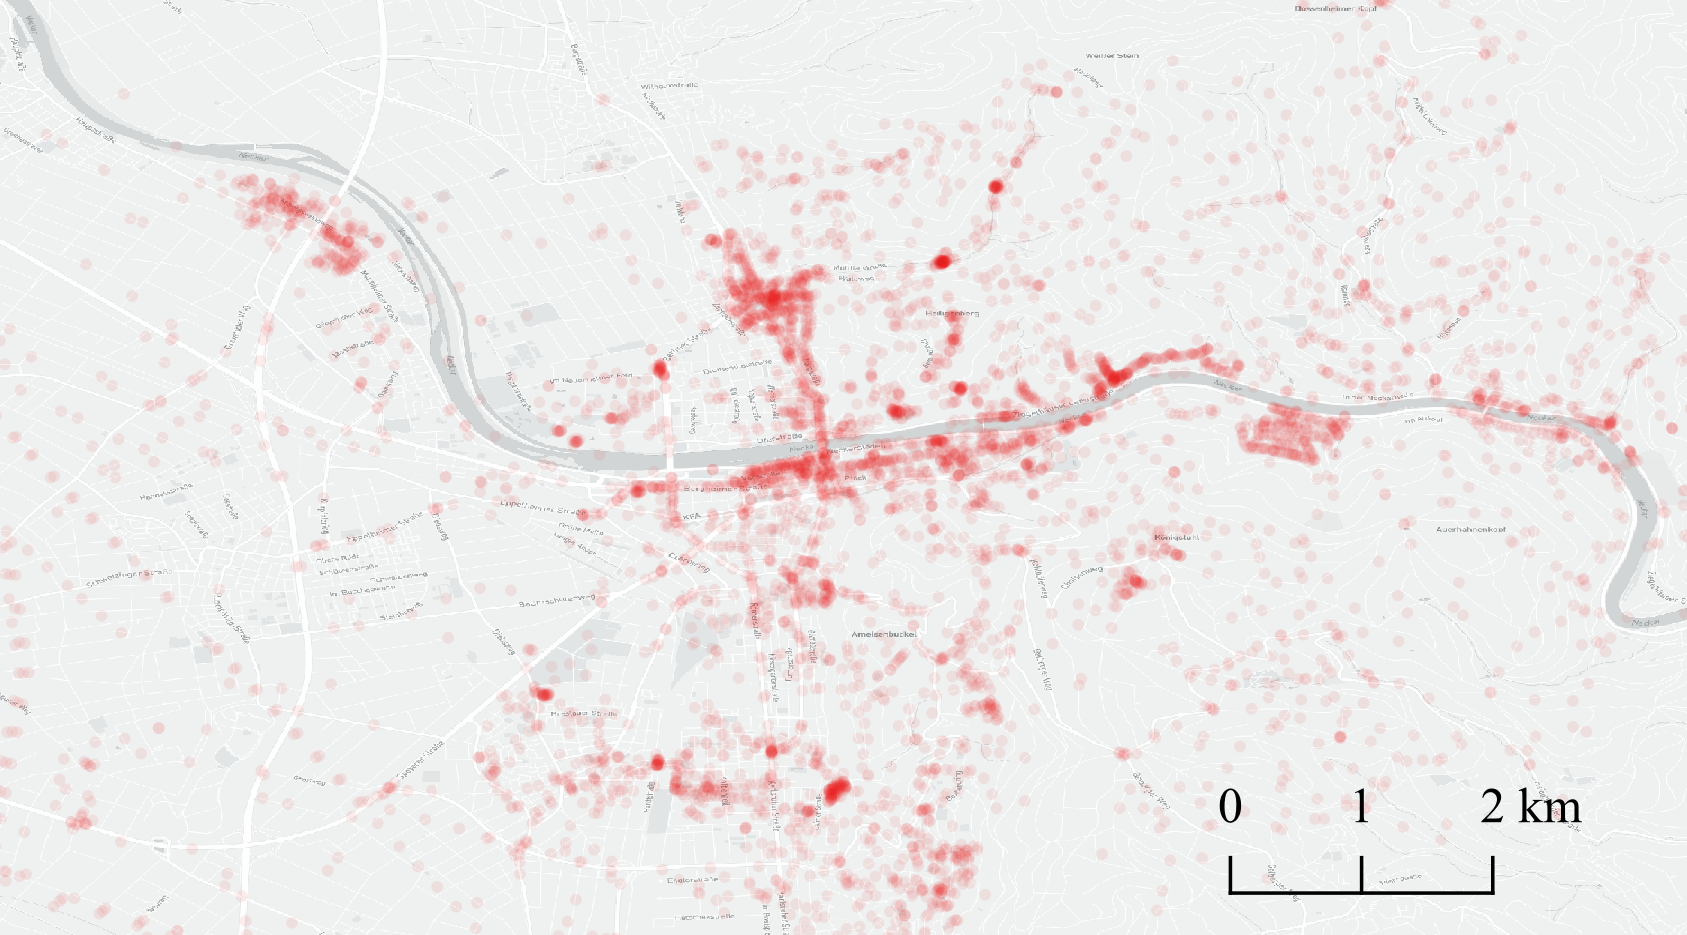
\includegraphics[width = \textwidth]{Images/hed_2.png} %this tells latex what graphics to include. 
    \caption{Spatial distribution of features mapped in Heidelberg case study} % this prints the caption below the figure
\end{figure}
%%%%%%%%%%%%%%%%%%%%%%%%%%


%%%%%%%%%%%%%%%%%%%%%%%%%% Tot maintenance
\begin{figure} % opens the figure environment. the '[H]' forces the image to be Here
    \centering % puts the image in the horizontal centre of the page
    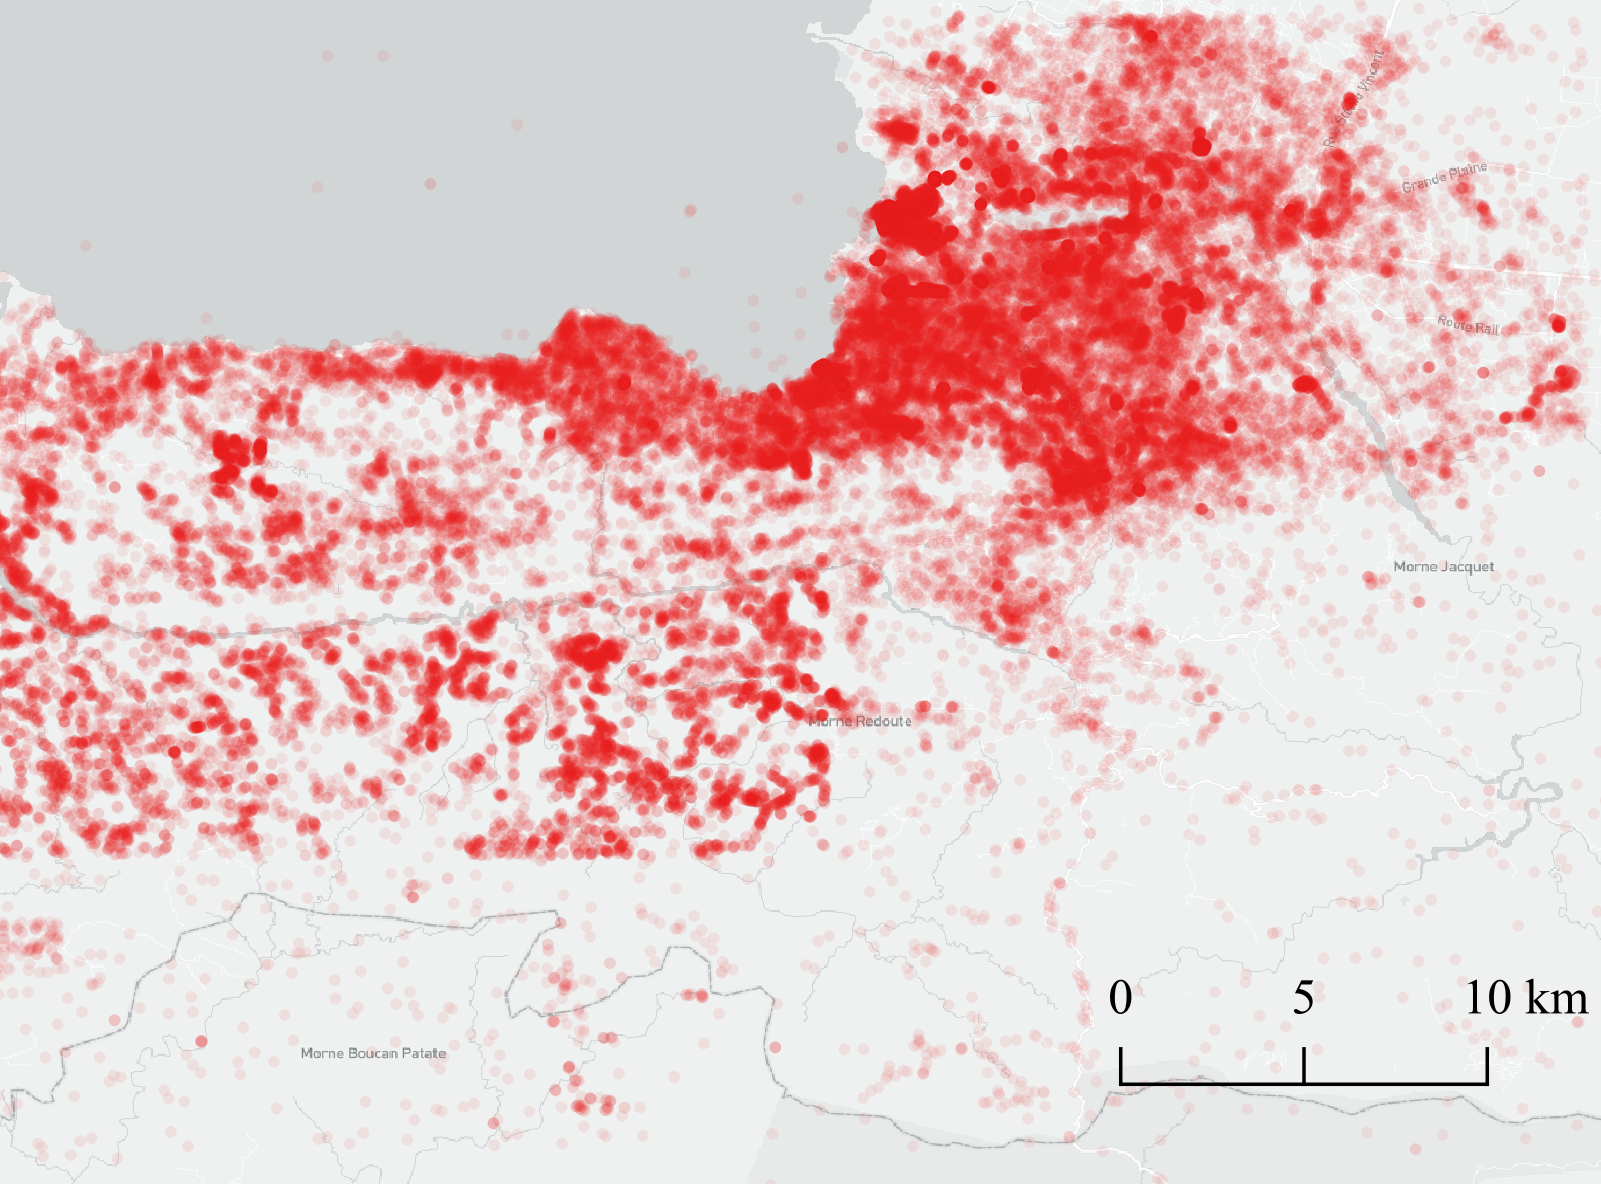
\includegraphics[width = \textwidth]{Images/pap_2.png} %this tells latex what graphics to include. 
    \caption{Spatial distribution of features mapped in Port au Prince case study} % this prints the caption below the figure
\end{figure}
%%%%%%%%%%%%%%%%%%%%%%%%%%

%%%%%%%%%%%%%%%%%%%%%%%%%% Tot maintenance
\begin{figure} % opens the figure environment. the '[H]' forces the image to be Here
    \centering % puts the image in the horizontal centre of the page
    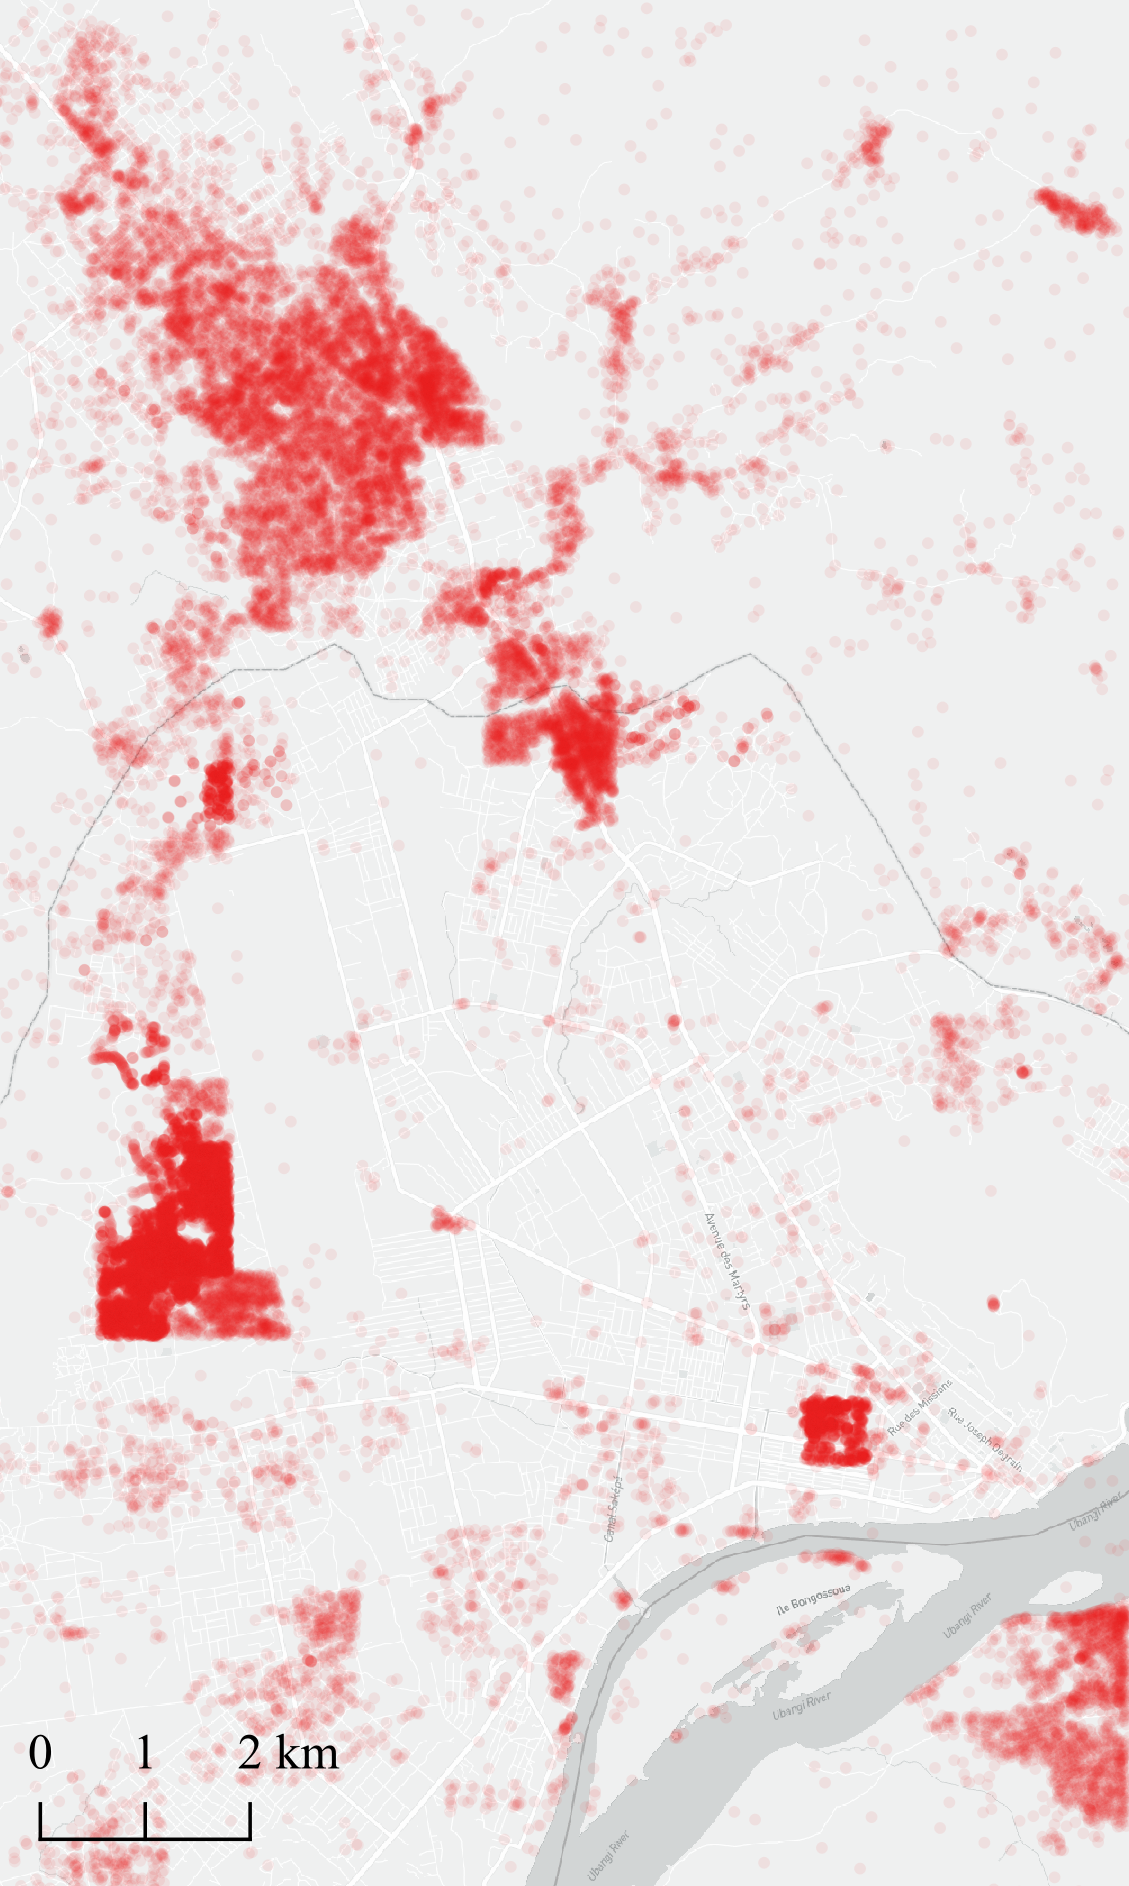
\includegraphics[width = \textwidth]{Images/car_2.png} %this tells latex what graphics to include. 
    \caption{Spatial distribution of features mapped in Bangui case study} % this prints the caption below the figure
\end{figure}
%%%%%%%%%%%%%%%%%%%%%%%%%%

%%%%%%%%%%%%%%%%%%%%%%%%%% Tot maintenance
\begin{figure} % opens the figure environment. the '[H]' forces the image to be Here
    \centering % puts the image in the horizontal centre of the page
    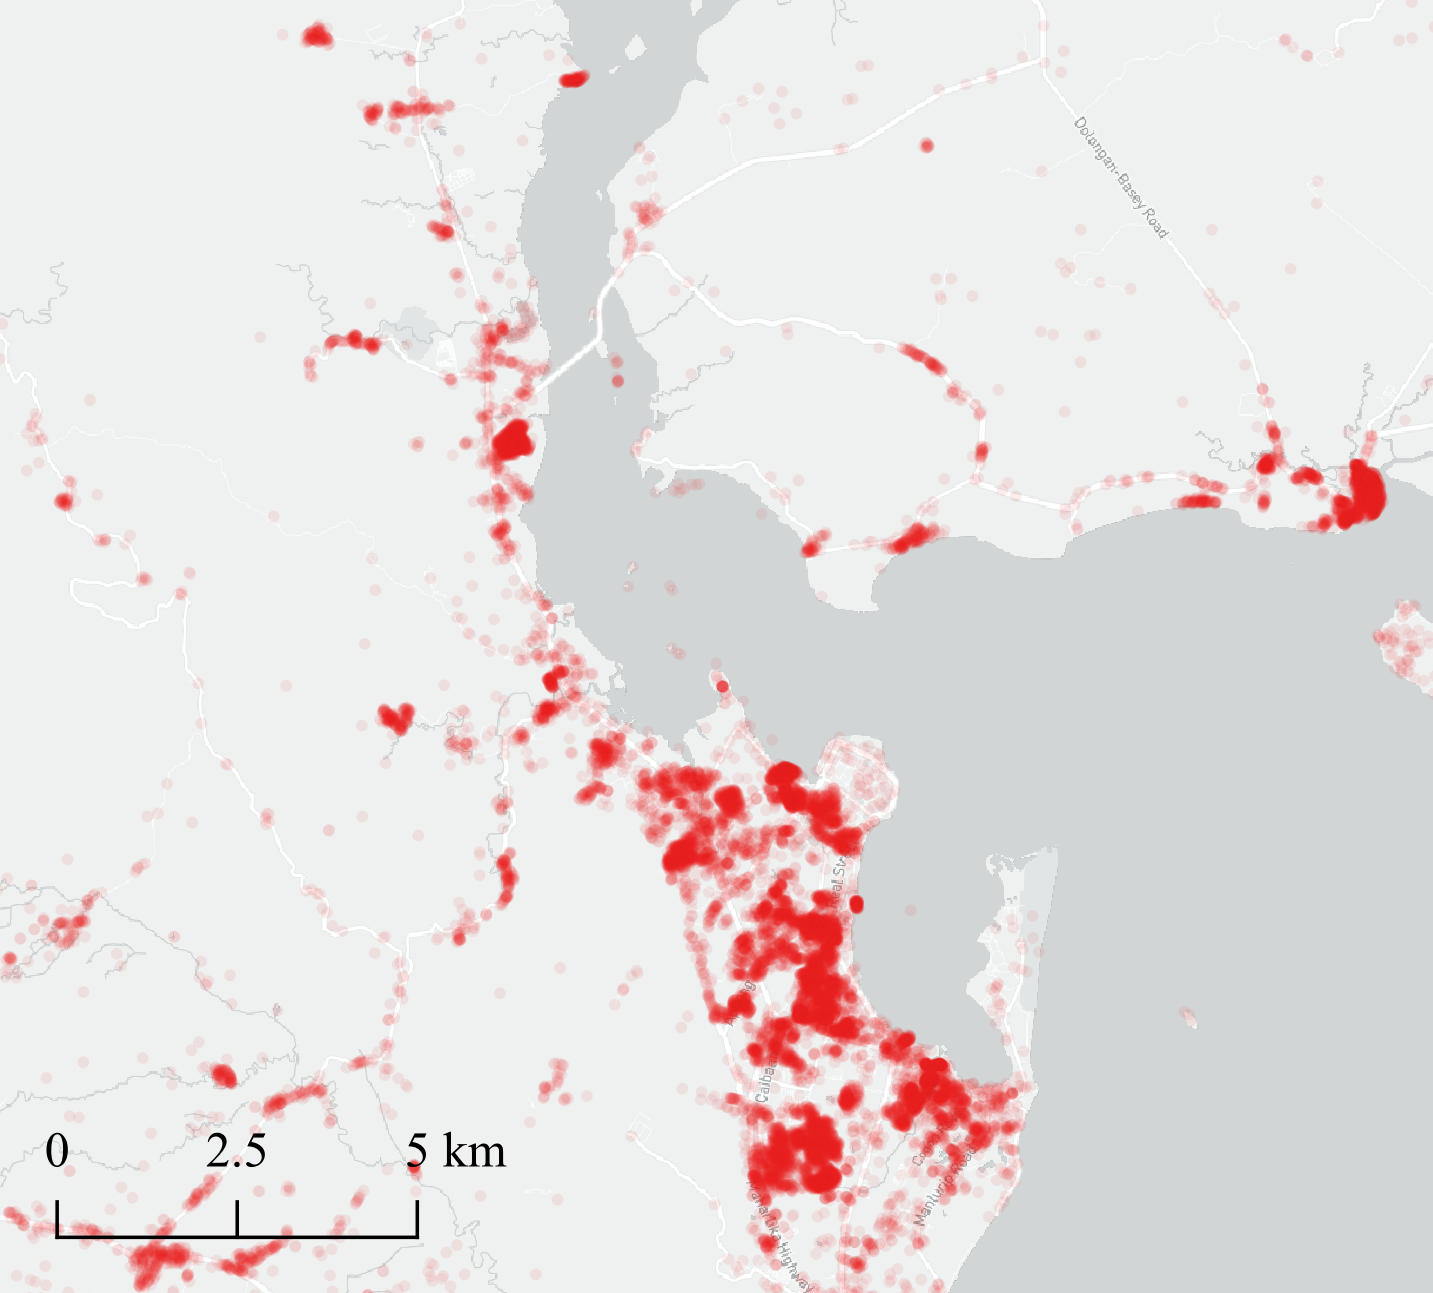
\includegraphics[width = \textwidth]{Images/tac_2.png} %this tells latex what graphics to include. 
    \caption{Spatial distribution of features mapped in Tacloban case study} % this prints the caption below the figure
\end{figure}
%%%%%%%%%%%%%%%%%%%%%%%%%%

%%%%%%%%%%%%%%%%%%%%%%%%%% Tot maintenance
\begin{figure} % opens the figure environment. the '[H]' forces the image to be Here
    \centering % puts the image in the horizontal centre of the page
    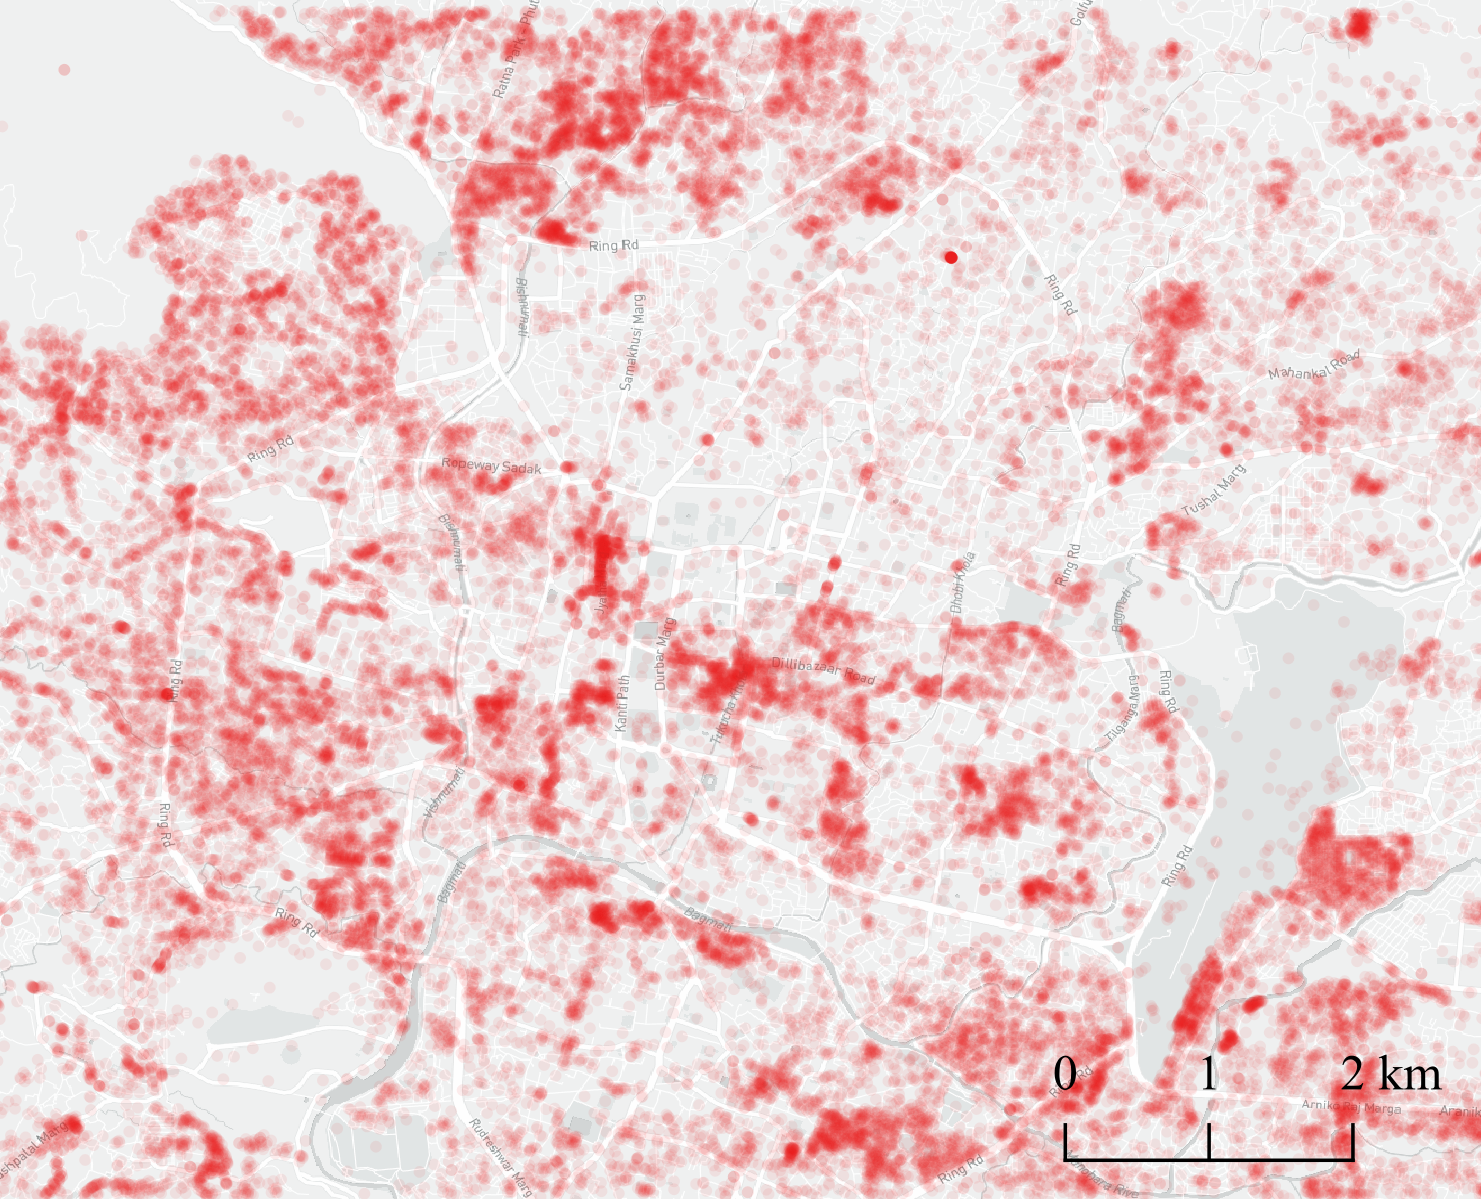
\includegraphics[width = \textwidth]{Images/nep_2.png} %this tells latex what graphics to include. 
    \caption{Spatial distribution of features mapped in Kathmandu case study} % this prints the caption below the figure
\end{figure}
%%%%%%%%%%%%%%%%%%%%%%%%%%
\chapter{Research Log}
\label{appendixlabel2}

This appendix contains documentation of this research process.

\begin{table}[H]
\centering
\begin{tabular}{ll} 
\hline
Date                                     & Notes                                                                                                                                                                                                \\ 
\hline
\rowcolor[rgb]{0.894,0.894,0.894} April  & \begin{tabular}[c]{@{}>{\cellcolor[rgb]{0.894,0.894,0.894}}l@{}}Begin to frame research topic; awaiting confirmation of \\support from MSF\end{tabular}                                                     \\
April 16th                               & \begin{tabular}[c]{@{}l@{}}Initial check-in meeting with Sarah to discuss research \\aims\end{tabular}                                                                                                      \\
April 21st                               & \begin{tabular}[c]{@{}l@{}}Meeting with Sarah and Jorieke (of MSF) to discuss \\potential support\end{tabular}                                                                                              \\
April 27th                               & Confirmation of support from MSF                                                                                                                                                                            \\
\rowcolor[rgb]{0.894,0.894,0.894} May    & \begin{tabular}[c]{@{}>{\cellcolor[rgb]{0.894,0.894,0.894}}l@{}}Begin literature review and design methodology; challenges \\managing heavy workload with submissions from other \\coursework\end{tabular}  \\
May 4th                                  & Review initial conceptual framework for project with Sarah                                                                                                                                                  \\
May 13th                                 & Begin draft literature review                                                                                                                                                                               \\
May 21st                                 & Kick-off meeting with MSF to discuss project ideas                                                                                                                                                          \\
\rowcolor[rgb]{0.894,0.894,0.894} June   & \begin{tabular}[c]{@{}>{\cellcolor[rgb]{0.894,0.894,0.894}}l@{}}Prepare draft literature review and methods proposal; \\personal challenges in relocating back to UK from Canada\end{tabular}               \\
June 4th                                 & \begin{tabular}[c]{@{}l@{}}Reviewed proposed Gantt chart for project with Sarah and \\discussed timeline for feedback\end{tabular}                                                                          \\
June 24th                                & \begin{tabular}[c]{@{}l@{}}Check in meeting with Jorieke (MSF) regarding initial \\findings from literature review\end{tabular}                                                                             \\
June 26th                                & Technical challenges in setting up local OSHDB database                                                                                                                                                     \\
June 30th                                & \begin{tabular}[c]{@{}l@{}}Meeting with Sarah to review key points from literature \\review and help to troubleshoot technical challenges\end{tabular}                                                      \\
\hline
\end{tabular}
\end{table}


\begin{table}[H]
\centering
\begin{tabular}{ll} 
\hline
Date                                     & Notes                                                                                                                                                                                                \\ 
\hline
\rowcolor[rgb]{0.894,0.894,0.894} July   & Conduct analysis and draft content for results                                                                                                                                                              \\
July 3rd                                 & \begin{tabular}[c]{@{}l@{}}Deliver draft literature review and methods roadmap to \\Sarah for review\end{tabular}                                                                                           \\
July 9th                                 & Received feedback from Sarah on draft material                                                                                                                                                              \\
July 29th                                & \begin{tabular}[c]{@{}l@{}}Meeting with Sarah to review preliminary results and \\discuss implications of findings\end{tabular}                                                                             \\
July 31st                                & Deliver draft results and discussion to Sarah for review                                                                                                                                                    \\
\rowcolor[rgb]{0.894,0.894,0.894} August & Focus on writing the dissertation document                                                                                                                                                                  \\
August 3rd                               & Received feedback from Sarah on draft material                                                                                                                                                              \\
August 19th                              & Check in with Sarah to review document structure and style                                                                                                                                                  \\
\hline
\end{tabular}
\end{table}

